\chapter{Ablation Study}
\label{ch:ablation}

Our proposed framework for knowledge graph fact verification utilizes a unique combination of web search and language model processing.
However, to ensure the robustness and effectiveness of our approach, it is crucial to compare our methods with state-of-the-art RAG techniques, particularly in the critical areas of chunking, embedding, and retrieval.

This section aims to provide a comprehensive comparison between our approach and the RAG-based methods proposed in recent literature.
We will focus on three key components of our framework: 1) the chunking strategies used to segment information, 2) the embedding models employed for representation, and 3) the retrieval mechanisms utilized to fetch relevant information.
By analyzing these components in light of RAG recommendations, we aim to identify potential areas for improvement and validate the strengths of our current approach.

Through this comparison, we seek to situate our work within the broader context of retrieval-augmented fact verification systems and provide insights into the trade-offs and benefits of our methodological choices.
This analysis will not only contribute to the refinement of our framework but also offer valuable perspectives on the application of RAG principles to knowledge graph fact verification tasks.


\section{Evaluation Methodology}\label{sec:evaluation-methodology}
This study employs a systematic approach to evaluate and optimize various components of our framework, with the ultimate goal of determining the best methods for each section.
Our methodology is designed to isolate and assess the impact of different techniques and parameters on overall system performance, while also considering the efficacy of sampling methods compared to full data runs.

\subsection{Iterative Optimization Process}\label{subsec:iterative-optimization-process}
The evaluation process follows an iterative strategy, focusing on specific sections of the framework in each iteration:

\begin{enumerate}
    \item \textbf{Section Isolation:} In each iteration, we isolate a particular section of the framework for investigation, keeping other components constant.
    This \("\)enclosed box\("\) approach allows for a controlled examination of individual elements.
    \item \textbf{Parameter Variation:} Within the isolated section, we systematically vary relevant parameters or methods.
    This includes, but is not limited to, testing different sampling methods against full data runs.
    \item \textbf{Performance Evaluation:} For each configuration, we assess the system's performance using predefined metrics (detailed in Section \ref{sec:metrics}).
    \item \textbf{Best Method Selection:} Based on the evaluation results, we identify the best-performing method or configuration for the section under investigation.
    \item \textbf{Incremental Optimization:} The optimal configuration from each iteration is incorporated into the framework for subsequent iterations, gradually refining the entire system.
\end{enumerate}

\subsection{Sampling Methods Evaluation}\label{subsec:sampling-methods-evaluation}

As one of the parameters under investigation, we compare various sampling methods to full data runs:

\begin{itemize}
    \item \textbf{Full Data Runs:} Establish a baseline using the entire dataset.
    \item \textbf{Simple Random Sampling:} Randomly select a subset of $n$ data points from a population of size $N$.
    \item \textbf{Unique Over Sampling:} Evenly distributes a specified number of samples across different categories in a dataset. It ensures minimal duplication by prioritizing unique samples and filling the remainder slots using random sampling when necessary.
\end{itemize}
This comparison aims to determine if sampling can reduce computational costs and accelerate results without significant loss in accuracy.

\subsection{Evaluation Metrics}
\label{sec:metrics}

The performance of each configuration is assessed using the following metrics:

\begin{itemize}
    \item \textbf{Accuracy (Acc):} Measures the overall correctness of predictions:
    \begin{equation}
        \text{Acc} = \frac{\text{TP} + \text{TN}}{\text{TP} + \text{TN} + \text{FP} + \text{FN}}
    \end{equation}
    where TP, TN, FP, and FN are True Positives, True Negatives, False Positives, and False Negatives, respectively.

    \item \textbf{F1 Score:} Provides a balanced measure of precision and recall:
    \begin{equation}
        \text{F1} = 2 \cdot \frac{\text{Precision} \cdot \text{Recall}}{\text{Precision} + \text{Recall}}
    \end{equation}

    \item \textbf{Average Score (Avg):} Calculated based on accuracy across multiple runs:
    \begin{equation}
        \text{Avg} = \frac{1}{m} \sum_{i=1}^m \text{Acc}_i
    \end{equation}
    where $m$ is the number of runs.

    \item \textbf{Average Latency:} Measured in seconds per query to assess computational efficiency:
    \begin{equation}
        \text{Avg Latency} = \frac{\text{Total Processing Time}}{\text{Number of Queries}}
    \end{equation}
\end{itemize}

\subsection{Significance of the Methodology}

This methodical approach serves several key purposes:

\begin{enumerate}
    \item \textbf{Optimization of Individual Components:} By isolating sections, we can fine-tune each part of the framework independently.
    \item \textbf{Holistic System Improvement:} The iterative process ensures that optimizations in one section complement the overall system performance.
    \item \textbf{Efficiency-Accuracy Trade-off Analysis:} Comparing sampling methods to full data runs helps balance computational efficiency with result accuracy.
    \item \textbf{Scalability Assessment:} This approach informs decisions on system scalability as data volumes increase.
\end{enumerate}

By employing this rigorous evaluation methodology, we aim to identify the best methods for each section of our framework, potentially enabling more efficient and accurate data processing.
The inclusion of sampling method comparisons adds an extra dimension to our optimization efforts, potentially offering insights into cost-effective alternatives to full data processing where applicable.



\section{Document Selection}\label{sec:document-selection}
We explore various techniques for retrieving relevant documents from search engine results, with a specific focus on Google search engine.
The goal is to identify the most effective methods for finding documents that perfectly match the information need expressed in the query.
We consider both unsupervised and supervised approaches.

\subsection{Unsupervised Methods}\label{subsec:unsupervised-methods}

\subsubsection{BM25}
BM25 is a widely used unsupervised retrieval method that relies on term frequency and inverse document frequency (TF-IDF) weighting.
It estimates the relevance of documents to a query based on the frequency of query terms in each document, offset by the rarity of those terms across the full document collection.
BM25 has proven to be a robust baseline for many retrieval tasks.
However, it relies on lexical matching between query and document terms, which can limit its effectiveness for queries and documents that use different vocabulary to express similar concepts.

\begin{algorithm}
    \caption{BM25-based Sentence Retrieval}
    \begin{algorithmic}[1]
        \Procedure{Preprocess}{sentence}
            \State Convert sentence to lowercase
            \State Remove punctuation
            \State Tokenize sentence into words
            \State Remove stopwords
            \State \Return preprocessed tokens
        \EndProcedure

        \Procedure{FetchSimilarSentences}{sentences, top\_n}
            \For{each sentence in sentences}
                \State preprocessed $\gets$ Preprocess(sentence)
                \State Add preprocessed to tokenized\_sentences
            \EndFor

            \State bm25 $\gets$ CreateBM25Object(tokenized\_sentences)
            \State query $\gets$ tokenized\_sentences[0]

            \State scores $\gets$ bm25.GetScores(query)
            \State Sort scored\_sentences by score in descending order

            \State result $\gets$ Top top\_n sentences from result

        \EndProcedure
    \end{algorithmic}
\end{algorithm}

\subsubsection{Contriever}
Contriever is a more recently proposed unsupervised method by Izacard et al.\cite{izacard2022unsuperviseddenseinformationretrieval} that leverages contrastive learning to train dense retrieval models.
Rather than relying on term matching, Contriever learns to map semantically similar text pairs to nearby embeddings in a continuous vector space.
At query time, Contriever embeds the query and retrieves the documents whose embeddings are nearest to the query under cosine similarity.
By operating in this learned semantic space, Contriever can potentially identify relevant documents that use different surface forms than the query.
Contriever has shown promising results, outperforming BM25 on a range of benchmarks when large unsupervised pretraining datasets are available.
However, details on its performance in this specific multi-query retrieval setup are needed to fully assess its capabilities here.

While Contriever can be used as an unsupervised retriever, for our thesis project focusing on search-related data, we opt to use the MS-MARCO fine-tuned version. \footnote{\url{https://huggingface.co/facebook/contriever-msmarco}}
Here's why:
\begin{itemize}
    \item \textbf{Relevance to Search Tasks:} MS-MARCO (Microsoft Machine Reading Comprehension) is a large-scale dataset specifically designed for search and question-answering tasks. It contains real queries from Bing search engine and human-annotated relevant passages. By fine-tuning Contriever on MS-MARCO, the model becomes particularly adept at understanding and representing search-like queries and documents.
    \item \textbf{Improved Performance:} Fine-tuning on MS-MARCO significantly boosts Contriever's performance on various retrieval benchmarks, especially those related to web search and question answering. This improvement is crucial for our project, which deals with search-term related data.
    \item \textbf{Domain Adaptation:} Although Contriever's unsupervised training on Wikipedia and CCNet provides a strong foundation, fine-tuning on MS-MARCO helps adapt the model to the specific nuances and patterns present in search queries and web documents. This domain adaptation is valuable for our search-centric application.
\end{itemize}

\subsection{Supervised Methods}\label{subsec:supervised-methods}

\subsubsection{Jina.ai Reranker}
The Jina.ai Reranker is a supervised neural ranking model.
Jina Reranker employs a cross-encoder architecture, which represents a paradigm shift from traditional bi-encoder models used in embedding-based search.
While bi-encoder models separately encode queries and documents, cross-encoders jointly process query-document pairs, allowing for more nuanced semantic understanding and relevance assessment.
The model generates a relevance score for each query-document pair, enabling a more precise ranking of search results.
This approach addresses limitations of vector similarity-based methods by capturing complex token-level interactions between queries and documents.

For our project, we use \textit{jina-reranker-v2-base-multilingual}\footnote{\url{https://huggingface.co/jinaai/jina-reranker-v2-base-multilingual}}.
This model has demonstrated exceptional performance across various benchmarks and practical applications.
In multilingual tasks, it achieved state-of-the-art recall@10 scores on the MKQA dataset \cite{mkqa} spanning 26 languages, while also exhibiting superior NDCG@10 scores on English-language tasks in the BEIR benchmark \cite{thakur2021beirheterogenousbenchmarkzeroshot}.
Notably, it secured the top position on the AirBench leaderboard upon its release \footnote{\url{https://huggingface.co/spaces/AIR-Bench/leaderboard}}.

These capabilities make the model particularly valuable for multilingual information retrieval, agentic Retrieval-Augmented Generation (RAG) systems, and even in programming and software development support.

\subsubsection{MS MARCO MiniLM}
The MS MARCO MiniLM is another supervised neural model, based on the popular BERT architecture but distilled to a smaller size for efficiency.

\begin{table}[ht!]
    \centering
    \noindent
    \resizebox{\textwidth}{!}{
        \begin{tabular}{lccc}
            \toprule
            \textbf{Model Name}      & \shortstack{\textbf{NDCG@10} \\ (TREC DL 19)} & \shortstack{\textbf{MRR@10} \\ (MS Marco Dev)} & \textbf{Docs / Sec} \\
            \midrule
            ms-marco-TinyBERT-L-2-v2 & 69.84                         & 32.56                          & 9000                \\
            ms-marco-MiniLM-L-2-v2   & 71.01                         & 34.85                          & 4100                \\
            ms-marco-MiniLM-L-4-v2   & 73.04                         & 37.70                          & 2500                \\
            ms-marco-MiniLM-L-6-v2   & 74.30                         & 39.01                          & 1800                \\
            ms-marco-MiniLM-L-12-v2  & 74.31                         & 39.02                          & 960                 \\
            \bottomrule
        \end{tabular}}
    \caption{Performance of Pre-trained Cross-Encoders}
    \label{tab:table2}
\end{table}

For our project, we use \textit{ms-marco-MiniLM-L-6-v2}\footnote{\url{https://huggingface.co/cross-encoder/ms-marco-MiniLM-L-6-v2}} Cross-Encoder model.
This model, trained on the extensive MS MARCO dataset comprising approximately 500,000 authentic search queries from the Bing search engine \cite{reimers-2019-sentence-bert}, demonstrates superior performance within a two-stage Retrieve \& Re-rank framework.
In this paradigm, an initial retrieval phase employs either lexical search methods or dense retrieval techniques utilizing a bi-encoder to identify a broad set of potentially relevant documents.
Subsequently, the Cross-Encoder refines this candidate set through a simultaneous processing of the query and each retrieved document, generating a relevance score on a scale of 0 to 1.

\subsection{Evaluation with Large Language Models}\label{subsec:evaluation-with-large-language-models}
With checking the similarity between the retrieved documents and the query in different methods, based on figure \ref{fig:document_retrieval_confusion_matrix} we can figured out that Bm25-Okapi stands out as the most distinct model, with low similarity scores (0.16-0.19) to the others, suggesting it employs fundamentally different retrieval mechanisms.
In contrast, the neural models show higher inter-model similarities (0.29-0.43), indicating shared approaches or architectures.
The strongest relationship (0.43) is between contriever-msmarco and re-ranker-msmarco, likely due to shared training data or similar optimizations.
The two re-ranker models also show high similarity (0.41), suggesting comparable re-ranking strategies.
In general, we can find out with different methods we have different result over the same query.

\begin{figure}[ht!]
    \centering
    \begin{minipage}[b]{0.45\textwidth}
        \centering
        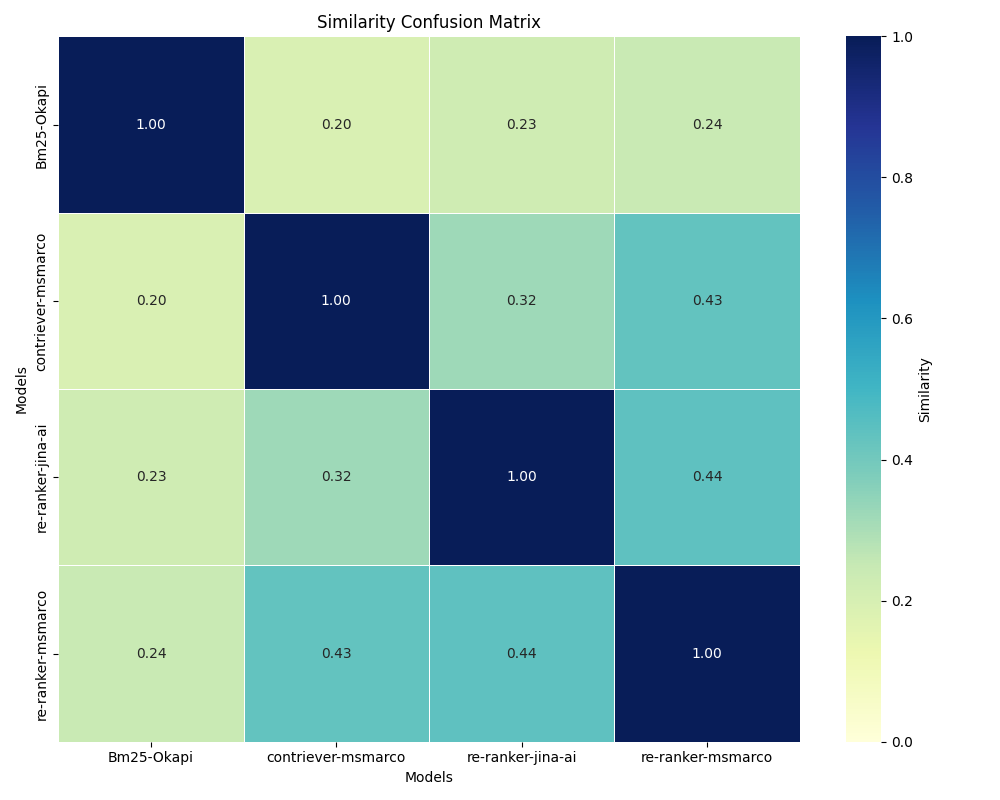
\includegraphics[width=\textwidth]{res/ret_result_sim_1.png}
        \caption{Document Retrieval Confusion Matrix}
        \label{fig:document_retrieval_confusion_matrix_1}
    \end{minipage}
    \hspace{0.05\textwidth} % Space between the images
    \begin{minipage}[b]{0.45\textwidth}
        \centering
        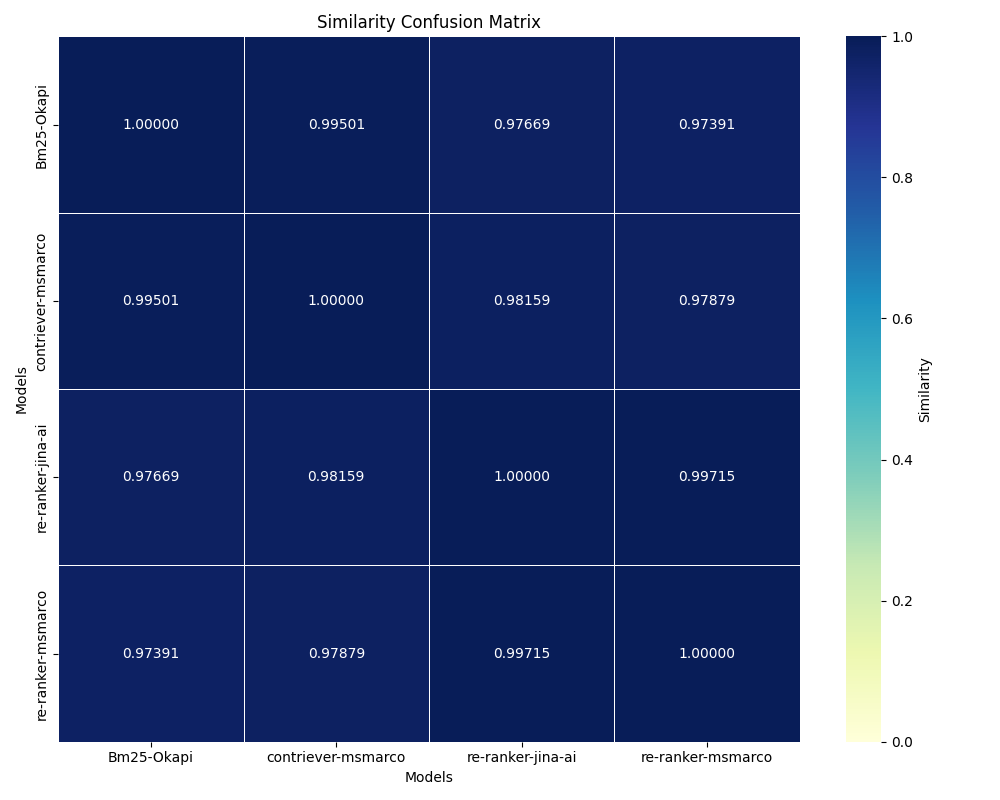
\includegraphics[width=\textwidth]{res/ret_result_sim_2.png}
        \caption{Document Retrieval Performance}
        \label{fig:document_retrieval_confusion_matrix_2}
    \end{minipage}
\end{figure}

To assess the quality of the retrieved documents from each of the above methods, we are passing them through one of our models and evaluating the outputs.

\begin{table}[h!]
    \noindent
    \resizebox{\textwidth}{!}{
        \begin{tabular}{cccccc||ccc}
            \multicolumn{9}{c}{\fbox{\textit{Retrieval Method}}, BAAI/bge-small-en-v1.5, Sliding Window - 6 , With Similarity Cut-off} \\ \\
            \multirow{2}{*}{\textbf{Method}} & \multicolumn{2}{c}{\textbf{Random Sampling}} & \textbf{Over Sampling} & \multicolumn{2}{c||}{\textbf{Avg.}} & \multicolumn{3}{c}{\textbf{Complete Run}} \\
            \cmidrule(lr){2-3}  \cmidrule(lr){4-4} \cmidrule(lr){5-6} \cmidrule(lr){7-9} \
            & Acc & F1 & Acc & Acc & \multicolumn{1}{c||}{F1} & Acc & F1 & Latency \\
            \midrule
            \multicolumn{1}{l}{\textit{Unsupervised}} & & & & & & & & \\
            \multicolumn{1}{l}{Bm25} & 0.719 & 0.505  & \textbf{0.450} & \textbf{0.212} & \multicolumn{1}{c||}{0.255} & 0.8882 & 0.8940 & 0.353\\
            \multicolumn{1}{l}{contriever-msmarco} & 0.505 & \textbf{0.450} & \textbf{0.212}  & \textbf{0.528} & \multicolumn{1}{c||}{0.255} & 0.8932 & 0.8988 & 0.353 \\
            \hdashline
            \multicolumn{1}{l}{\textit{supervised}} & & & & & & & & \\
            \multicolumn{1}{l}{jina-reranker-v2-base-multilingual} & 0.719  & \textbf{0.450} & \textbf{0.212} & 0.255  & \multicolumn{1}{c||}{0.255} & 0.9004 & 0.9065 & 0.9065\\
            \multicolumn{1}{l}{ms-marco-MiniLM-L-6-v2} & 0.719 & 0.505 & \textbf{0.450} & \textbf{0.212} & \multicolumn{1}{c||}{0.255} & \textbf{0.9014} & \textbf{0.9077} & 0.353\\
            \bottomrule
        \end{tabular}}\caption{Evaluation Results for Different Methods through the Pipeline (just with the Gemma2 model)}
    \label{tab:evaluation_results}
\end{table}

The empirical results indicate that the model \textit{ms-marco-MiniLM-L-6-v2} achieved the highest F1 score, thus demonstrating superior performance among the evaluated models.
However, it is noteworthy that the performance metrics across all models were closely clustered, suggesting that even traditional methodologies applied within our pipeline yield satisfactory outcomes.

It is crucial to emphasize the significance of data quality in this context, as it substantially influences the efficacy of the results.
To validate the factual accuracy of the knowledge graph, we employed a multi-query information fetching through web search engines for each fact.
This approach provides a reasonable degree of verification for the facts contained within the knowledge graph.

For subsequent evaluations and analyzes, we will designate the model \textit{ms-marco-MiniLM-L-6-v2} as our baseline for retrieval tasks.
This decision is predicated on its superior F1 score relative to the other models under consideration.


\section{Embedding Models}\label{sec:embedding-models}
Text embeddings are dense vector representations that capture the semantic meaning and relationships between words, sentences, or documents in a low-dimensional space.
By mapping text to a continuous vector space, embeddings enable efficient similarity computations and have become a fundamental building block for many natural language processing (NLP) applications, such as information retrieval, text classification, clustering, and semantic search.
This section provides an in-depth analysis and comparison of five state-of-the-art text embedding models:

\begin{itemize}
    \item Alibaba-NLP/gte-large-en-v1.5
    \item jinaai/jina-embeddings-v3
    \item dunzhang/stella\_en\_1.5B\_v5
    \item Nextcloud-AI/multilingual-e5-large-instruct
    \item BAAI/bge-small-en-v1.5
\end{itemize}

These models leverage recent advancements in transformer architectures, contrastive learning, and instruction fine-tuning to produce high-quality, general-purpose embeddings that excel across a wide range of downstream tasks.
We examine their model architectures, training methodologies, supported features, and empirical performance on standard benchmarks.
Through this comparative study, we aim to provide insights and guidance for practitioners to select the most suitable embedding model based on their specific use case and computational constraints.

\subsection{Alibaba-NLP/gte-large-en-v1.5}\label{subsec:alibaba-nlp}

\subsubsection{Model Overview}
The gte-large-en-v1.5 model is part of the gte-vl.5 series released by the Institute for Intelligent Computing at Alibaba Group [Zhang et al., 2023].
It is built upon a transformer++ encoder backbone, which enhances the standard BERT architecture [Devlin et al., 2018] with rotary position embeddings (RoPE) [Su et al., 2021] and gated linear units (GLU) [Dauphin et al., 2017].
The model supports input sequences up to 8192 tokens, a significant improvement over previous multilingual encoders limited to 512 tokens.

\subsubsection{Training Methodology}
gte-large-en-v1.5 undergoes a three-stage training pipeline:
\begin{itemize}
    \item Masked language modeling (MLM) pre-training on the C4 dataset
    \item Weakly-supervised contrastive pre-training on GTE pre-training data
    \item Supervised contrastive fine-tuning on GTE fine-tuning data
\end{itemize}

The MLM pre-training follows a two-stage curriculum to efficiently handle long sequences.
It first trains on shorter 512 token inputs, then resamples the data to include more long sequences and continues MLM on 8192 token inputs.
The contrastive pre-training and fine-tuning stages utilize diverse text pair datasets to learn general-purpose text representations.

\subsubsection{Evaluation}
\textit{gte-large-en-v1.5} demonstrates strong performance on the MTEB multilingual benchmark, achieving state-of-the-art results in its model size category.
It also shows competitive results on the LoCo long-context retrieval benchmark.
The model strikes a good balance between embedding quality and computational efficiency.

\subsection{jinaai/jina-embeddings-v3}\label{subsec:jinaai}

\subsubsection{Model Overview}
jina-embeddings-v3 is a multilingual multi-task text embedding model developed by Jina AI [Sturm et al., 2023].
Based on the XLM-RoBERTa architecture [Conneau et al., 2019], it incorporates rotary position embeddings (RoPE) to handle input sequences up to 8192 tokens.
A key feature is the inclusion of 5 LoRA (low-rank adaptation) [Hu et al., 2021] adapters to efficiently generate task-specific embeddings for retrieval, clustering, classification, and text matching.

\subsubsection{Training Methodology}
jina-embeddings-v3 is first pre-trained using masked language modeling on a large multilingual corpus.
It then undergoes contrastive pre-training on weakly-supervised text pairs mined from web data.
inally, the model is fine-tuned using supervised contrastive learning on annotated datasets for specific tasks.
The training leverages recent techniques like Matryoshka embeddings [Kusupati et al., 2022] which allow flexibly truncating the embedding size to reduce storage costs.

\subsubsection{Evaluation}
On the MTEB benchmark, jina-embeddings-v3 outperforms other multilingual models like XLMR and achieves state-of-the-art results on several English tasks, surpassing large models from OpenAI and Cohere.
Its strong cross-lingual transfer and flexible embedding size options make it highly practical for real-world applications.

\subsection{dunzhang/stella\_en\_1.5B\_v5}\label{subsec:dunzhang}

\subsubsection{Model Overview}
stella\_en\_1.5B\_v5 is an English-specific embedding model built by Baai based on Alibaba's gte-large-en-vl.5 [Dunzhang, 2023]. It simplifies the usage of prompts, providing two general templates (one for sentence-to-passage and one for sentence-to-sentence tasks). Through Matryoshka representation learning, the model supports elastic embeddings with dimensions ranging from 32 to 8192, allowing users to easily trade off between embedding size and quality.

\subsubsection{Training Methodology}
stella\_en\_1.5B\_v5 follows a similar training pipeline as gte-large-en-v1.5, with masked language modeling pre-training, followed by weakly-supervised contrastive learning on large-scale web data. The contrastive fine-tuning stage incorporates supervision from diverse high-quality English datasets. Reversed RoPE scaling is employed during pre-training to handle longer sequences more efficiently.

\subsubsection{Evaluation}
stella\_en\_1.5B\_v5 achieves strong results on the SentEval and BEIR benchmarks, often outperforming larger models. The elastic embeddings provide significant flexibility - the 1024d and 512d options perform comparably to the full 8192d embeddings in most cases, while being much more efficient.

\subsection{Nextcloud-AI/multilingual-e5-large-instruct}\label{subsec:nextcloud-ai}

\subsubsection{Model Overview}
multilingual-e5-large-instruct is a multilingual extension of the E5 text embedding model [Wang et al., 2023].
It has 24 transformer layers and produces 1024-dimensional embeddings.
The model is initialized from XLM-RoBERTa-large and trained on a mixture of multilingual datasets with a focus on 30 languages.

\subsubsection{Training Methodology}
The training of multilingual-e5-large-instruct involves two main stages:
Contrastive pre-training on 1 billion weakly-supervised text pairs
Fine-tuning on datasets from the E5-mistral paper [Wang et al., 2023]
For the fine-tuning stage, each text pair is prepended with a one-sentence instruction describing the task (e.g. "Given a web search query, retrieve relevant passages that answer the query"). This instruction tuning setup allows the model to adapt its representations for different use cases.

\subsubsection{Evaluation}
multilingual-e5-large-instruct demonstrates strong performance on both monolingual and cross-lingual benchmarks like MKQA, MLDR, and BEIR. On several non-English datasets, it outperforms much larger models like mDPR and E5-mistral-7b. The instruction tuning proves highly effective in aligning the embeddings for specific tasks.

\subsection{BAAI/bge-small-en-v1.5}\label{subsec:baai}

\subsubsection{Model Overview}
The bge-small-en-v1.5 model is part of the BGE (BAAI General Embeddings) series developed by the Beijing Academy of Artificial Intelligence [Xiao et al., 2023]. It is a compact English-specific model with just 25M parameters, making it highly efficient for deployment in resource-constrained environments. The model architecture is based on RoBERTa [Liu et al., 2019] with optimizations like dynamic token pruning and embedding factorization to reduce computational costs.

\subsubsection{Training Methodology}
bge-small-en-v1.5 follows a two-stage training pipeline similar to other BGE models:

Weakly-supervised contrastive pre-training on large-scale web data
Supervised fine-tuning on a curated set of high-quality English NLP datasets

The pre-training stage leverages diverse data sources like Wikipedia, Reddit, and CommonCrawl to learn general-purpose text representations. The fine-tuning stage incorporates datasets spanning retrieval, classification, paraphrase detection, and semantic textual similarity tasks to instill task-specific knowledge.

\subsubsection{Evaluation}
Despite its small size, bge-small-en-v1.5 punches above its weight on several English benchmarks.
On the SentEval suite, it outperforms the base-sized BERT and RoBERTa models on most tasks while being 4x more compact.
On retrieval challenges like BEIR, it achieves competitive results, often surpassing larger models like MPNet and the original DPR.
The model's strong performance can be attributed to the efficient architecture design and the use of high-quality fine-tuning data.
It presents an attractive option for applications requiring low-latency inference or deployment on edge devices.

\subsection{Comparative Analysis}\label{subsec:comparative-analysis}

\subsubsection{Model Size and Efficiency}
The six models cover a broad spectrum of sizes, from the 25M parameter bge-small-en-v1.5 to the 7B parameter e5-multilingual-7b-instruct-v2. The smaller models (bge-small-en-v1.5, stella\_en\_1.5B\_v5) excel in scenarios with strict latency or memory constraints, while the larger models (e5-multilingual-7b-instruct-v2, gte-large-en-v1.5) provide maximum accuracy for offline processing or applications demanding the highest quality embeddings.
The base-scale models (jina-embeddings-v3, multilingual-e5-large-instruct) strike a good balance for most use cases, delivering strong performance with reasonable computational requirements. Notably, bge-small-en-v1.5 achieves impressive results despite its tiny size, making it a top choice for efficiency-focused applications.


\begin{table}[ht!]
    \centering
    \noindent
    \resizebox{\textwidth}{!}{
        \begin{tabular}{lcccc}
            \toprule
            \textbf{Model} & \shortstack{\textbf{Model Size} \\ (Million Parameters)}           & \shortstack{\textbf{Memory Usage} \\ (GB, fp32)}             & \shortstack{\textbf{Embedding}  \\ \textbf{Dimensions}}              & \shortstack{\textbf{Max}  \\ \textbf{Tokens}} \\
            \midrule
            stella\_en\_1.5B\_v5              & 1543   & 5.75 & 8192  & 131072  \\
            jina-embeddings-v3              & 572   & 2.13 & 1024  & 8194  \\
            gte-large-en-v1.5              & 434   & 1.62 & 1024  & 8192  \\
            multilingual-e5-large-instruct              & 560   & 2.09 & 1024  & 514  \\
            bge-small-en-v1.5              & 33   & 0.12 & 384  & 51262  \\
            \bottomrule
        \end{tabular}}
    \caption{Comparison of Embedding Models}
    \label{tab:comparison-embeddings}
\end{table}

\subsubsection{Language Coverage}
Three models (gte-large-en-v1.5, stella\_en\_1.5B\_v5, bge-small-en-v1.5) are designed specifically for English, while the others offer multilingual support. jina-embeddings-v3 covers 100+ languages with a focus on 30 major ones, and the E5 models support 100 languages but may see degraded performance on low-resource languages.
For English-only applications, the specialized models are recommended, with bge-small-en-v1.5 being the most efficient and gte-large-en-v1.5 providing the highest quality. jina-embeddings-v3 is a strong choice when both English performance and broad language coverage are desired.

\subsubsection{Supported Features}
All models handle long input sequences (≥2048 tokens), which is important for document-level tasks. jina-embeddings-v3 includes dedicated task-specific adapters for fine-grained control, while the E5 models leverage instruction prompts for easy task adaptation.
stella\_en\_1.5B\_v5 and jina-embeddings-v3 support Matryoshka embeddings for flexibly adjusting embedding sizes, and bge-small-en-v1.5 employs embedding factorization for better efficiency-quality trade-offs at low dimensions.

\subsubsection{Empirical Performance}
On English benchmarks, gte-large-en-v1.5 and stella\_en\_1.5B\_v5 generally lead the pack, followed closely by bge-small-en-v1.5 which punches far above its weight class. jina-embeddings-v3 also shows strong English results while supporting many more languages.
For multilingual tasks, e5-multilingual-7b-instruct-v2 achieves the highest absolute scores, while jina-embeddings-v3 and multilingual-e5-large-instruct offer the best performance-efficiency trade-offs.
On long-context understanding, the E5 models and gte-large-en-v1.5 are top choices, with bge-small-en-v1.5 and stella\_en\_1.5B\_v5 being less suitable due to their more limited sequence lengths.

\subsubsection{Conclusion}
In this extended comparative study, we analyzed five state-of-the-art text embedding models: gte-large-en-v1.5, jina-embeddings-v3, stella\_en\_1.5B\_v5, multilingual-e5-large-instruct, and bge-small-en-v1.5.
Key insights:

Model size presents a key trade-off: larger models offer maximum quality but at steep computational costs, while smaller models prioritize efficiency, with bge-small-en-v1.5 showing impressive performance-size ratio.
For English-only applications, the specialized gte-large-en-v1.5, stella\_en\_1.5B\_v5 and bge-small-en-v1.5 are top picks, while jina-embeddings-v3 and the E5 models are best for multilingual use cases.
Models with flexible embedding sizes (stella\_en\_1.5B\_v5, jina-embeddings-v3, bge-small-en-v1.5) enable powerful yet efficient representations for real-world applications.
Instruction prompts (E5 models) and dedicated task adapters (jina-embeddings-v3) offer convenient mechanisms for adapting embeddings to specific downstream tasks.
Empirically, all models show strong results on a wide range of benchmarks, with e5-multilingual-7b-instruct-v2 leading in absolute scores, gte-large-en-v1.5 and stella\_en\_1.5B\_v5 excelling at English understanding, and jina-embeddings-v3 providing an excellent balance for multilingual applications.

Selecting the right embedding model requires careful consideration of the target use case, available computational resources, and deployment constraints.
For English-centric applications prioritizing efficiency, bge-small-en-v1.5 is a top choice, while gte-large-en-v1.5 and stella\_en\_1.5B\_v5 deliver maximum quality.
jina-embeddings-v3 and the E5 models are recommended for scenarios requiring broad language coverage and task flexibility.
As text embedding techniques continue to advance at a rapid pace, this comparative analysis aims to provide a snapshot of the current state-of-the-art and offer practical insights for practitioners.
By understanding the strengths and trade-offs of each model, researchers and developers can make informed decisions when building embedding-powered applications.
Looking ahead, we expect to see further innovations in model efficiency, task adaptation, and cross-lingual transfer, unlocking even more powerful and versatile text representations.


\section{Chunking Strategies}\label{sec:chunking-strategies}
A critical component of \ac{RAG} systems is the chunking strategy employed to divide documents into smaller, manageable pieces for efficient retrieval and processing.
This chapter examines three distinct chunking methods for \ac{RAG} systems, each with its unique characteristics and potential advantages.

\subsection{Parsing Documents into Text Chunks (Nodes)}\label{subsec:parsing-documents-into-text-chunks}
The first method we will explore involves parsing documents into text chunks, also referred to as nodes, of fixed sizes.
This approach is straightforward and widely used in many RAG implementations.
We will investigate three different chunk sizes: 256, 512, and 1024 tokens.
\subsubsection{Methodology}
In this method, documents are sequentially divided into chunks of the specified size.
If the final chunk is smaller than the designated size, it is typically padded or left as is, depending on the implementation.
\subsubsection{Chunk Sizes}
\begin{itemize}
    \item 256-token chunks: This size offers fine granularity, potentially allowing for more precise retrieval of relevant information. However, it may result in a loss of context for more complex topics that require broader context.
    \item 512-token chunks: This medium-sized chunk strikes a balance between granularity and context preservation. It is often considered a good default choice for many applications.
    \item 1024-token chunks: Larger chunks preserve more context but may retrieve more irrelevant information and increase computational overhead during retrieval and processing.
\end{itemize}
\subsubsection{Advantages and Limitations}
Advantages:
\begin{enumerate}
    \item Simple to implement and understand
    \item Consistent chunk sizes facilitate uniform processing
\end{enumerate}
Limitations:
\begin{enumerate}
    \item Fixed chunk sizes may not align with natural breaks in the text
    \item Larger chunks can introduce irrelevant information and increase computational costs
\end{enumerate}
\subsection{Smaller Child Chunks Referring to Bigger Parent Chunks (Small2Big)}\label{subsec:smaller-child-chunks-referring-to-bigger-parent-chunks}
The second method, which we will refer to as \textit{Small2Big}, involves creating a hierarchical structure of chunks, where smaller child chunks refer to larger parent chunks.
This approach aims to combine the benefits of fine-grained retrieval with the context preservation of larger chunks.
\subsubsection{Methodology}
In this method, documents are parsed into three levels of chunks:
\begin{itemize}
    \item Smallest children: 128-token chunks
    \item Intermediate parents: 256-token chunks
    \item Largest parents: 512-token chunks
\end{itemize}
Each smaller chunk maintains a reference to its parent chunks, allowing the system to retrieve additional context when needed.
\subsubsection{Advantages and Limitations}
Advantages:
\begin{enumerate}
    \item Allows for fine-grained retrieval with the option to expand context
    \item Adapts to different levels of specificity required by queries
\end{enumerate}
Limitations:
\begin{enumerate}
    \item More complex to implement and manage
    \item Increased storage requirements due to redundancy in the hierarchy
\end{enumerate}
\subsection{Sentence Window Retrieval}\label{subsec:sentence-window-retrieval}
The third method, Sentence Window Retrieval, focuses on maintaining semantic coherence by chunking based on sentences and incorporating surrounding context through windows.
\subsubsection{Methodology}
In this approach, documents are first split into individual sentences.
For each sentence, a \textit{window} of surrounding sentences is included to provide context.
We will examine two window sizes: 3 and 6.
\subsubsection{Window Sizes}
\begin{itemize}
    \item Window Size 3: For each sentence, the chunk includes the sentence itself, one preceding sentence, and one following sentence.
    \item Window Size 6: For each sentence, the chunk includes the sentence itself, two preceding sentences, and three following sentences.
\end{itemize}
\subsubsection{Advantages and Limitations}
Advantages:
\begin{enumerate}
    \item Preserves semantic units (sentences) and their immediate context
    \item Adapts to the natural structure of the text
\end{enumerate}
Limitations:
\begin{enumerate}
    \item Variable chunk sizes may complicate processing and indexing
    \item Optimal window size may vary depending on the document type and content
\end{enumerate}
\subsection{Evaluation}\label{subsec:evaluation}
Each of the three chunking methods presented in this chapter offers distinct advantages and limitations for RAG systems. 
The choice of method depends on factors such as the nature of the documents, the specific requirements of the application, and the computational resources available.
The fixed-size chunking method provides simplicity and consistency but may sacrifice semantic coherence. 
The Small2Big hierarchical approach offers flexibility in retrieval granularity but introduces complexity in implementation and storage. 
Sentence Window Retrieval preserves semantic units and adapts to text structure but may result in variable chunk sizes.
\begin{table}[h!]
    \noindent
    \resizebox{\textwidth}{!}{
        \begin{tabular}{ll|ccccc||ccc}
            \multicolumn{10}{c}{\fbox{\textit{Retrieval Method}}, fdsjnfkdsn, jfiewdf ,fjneirufj} \\ \\
            \multirow{2}{*}{\textbf{Method}} & \multirow{2}{*}{\textbf{Parameters}} & \multicolumn{2}{c}{\textbf{Random Sampling}} & \textbf{Over Sampling} & \multicolumn{2}{c||}{\textbf{Avg.}} & \multicolumn{3}{c}{\textbf{Complete Run}} \\
            \cmidrule(lr){3-4} \cmidrule(lr){5-5} \cmidrule(lr){6-7} \cmidrule(lr){8-10}\
            & & Acc & F1 & Acc & Acc & \multicolumn{1}{c||}{F1} & Acc & F1 & Latency \\
            \midrule
            \multirow{3}{*}{Original} & Chuck Size: 1024 &  0.719  & 0.391 & \textbf{0.450} & \textbf{0.212} & \multicolumn{1}{c||}{0.255} & \textbf{0.528} & 0.353 & 0.353 \\
            & Chuck Size: 512 & 0.719 & 0.391 & \textbf{0.450} & \textbf{0.212} & \multicolumn{1}{c||}{0.255} & \textbf{0.528} & 0.353 & 0.353\\
            & Chuck Size: 256 & 0.719 & 0.505 & \textbf{0.450} & \textbf{0.212} & \multicolumn{1}{c||}{0.255} & \textbf{0.528} & 0.353 & 0.353\\
            \hdashline
            small2big & Text Chunks: 8 * 128, 4 * 256, 2 * 512 & 0.505 & 0.391 & \textbf{0.450} & \textbf{0.212} & \multicolumn{1}{c||}{0.255} & \textbf{0.528} & 0.353 & 0.353 \\
            \hdashline
            \multirow{2}{*}{Sliding Window} & Window Size: 6 &  0.719 & 0.505  & \textbf{0.450} & \textbf{0.212} & \multicolumn{1}{c||}{0.255} & \textbf{0.528} & 0.353 & 0.353 \\
            & Window Size: 3 & 0.719 & 0.505 & \textbf{0.450} & \textbf{0.212} & \multicolumn{1}{c||}{0.255} & \textbf{0.528} & 0.353 & 0.353 \\
            \bottomrule
        \end{tabular}}\caption{Evaluation Results for Different Embeddings Models through the Pipeline (just with the Gemma2 model)}
    \label{tab:table_chunking}
\end{table}
Examples of the three chunking methods are available in the appendix~\ref{ch:chunking} for further reference.

\section{Similarity Cut-off}\label{sec:similar-cut-off}
In this section we will discuss how similarity cut-off can be used to filter out irrelevant nodes and improve the efficiency of the retrieval process.
We use Node postprocessors to apply a similarity cut-off to the retrieved nodes, discarding those with a similarity score below a certain threshold.
Node postprocessors are a set of modules that take a set of nodes, and apply some kind of transformation or filtering before returning them.
For our experiments, we set the similarity cut-off threshold to 0.3, meaning that nodes with a similarity score below 0.3 are discarded, and also we re-rank the nodes based on their similarity score with re-ranker models (\textit{ms-marco-MiniLM-L-6-v2} and \textit{jina-reranker-v2-base-multilingual}) and not their original score.

\begin{algorithm}
    \begin{algorithmic}[1]
        \Procedure{PostprocessNodes}{nodes, knowledge\_graph, similarity\_cutoff}
            \State $new\_nodes \gets []$
            \State $node\_texts \gets [node.text \text{ for } node \text{ in } nodes]$
            \State $re\_rank\_nodes \gets \textsc{ReRank}(knowledge\_graph, node\_texts)$

            \For{each $node$ in $nodes$}
                \State $node.score \gets \text{get\_node\_score}(node.text, re\_rank\_nodes)$

                \If{$node.score > similarity\_cutoff$}
                    \State $new\_nodes.\textsc{Append}(node)$
                \EndIf
            \EndFor

            \State \Return $new\_nodes$
        \EndProcedure
    \end{algorithmic}
    \caption{Similarity Cutoff Postprocessor}\label{alg:algorithm}
\end{algorithm}

\section{Evaluation}\label{sec:evaluation-and-discussion}


\section{Failure Analysis}\label{sec:faiure-analysis}